% =============================================================
%  classical_thermodynamics.tex
%  IPhO 培訓用之古典熱力學講義。
%  本檔擬由 lecture.tex 以 \input 引入（此處沒有 \documentclass /
%  \begin{document}）。母檔應提供：
%      \usepackage{amsmath,amssymb,amsthm,mathtools}
%      \usepackage{bm}
%      \usepackage{enumitem}
%      （以及任何想要的定理環境定義）
% =============================================================

% --- 下方使用的速記指令 --------------------------------------
\providecommand{\dd}{\mathrm{d}}
\providecommand{\dbar}{\mathchar'26\mkern-12mu\mathrm{d}}  % 非恰當微分
\providecommand{\pd}[2]{\dfrac{\partial #1}{\partial #2}}
\providecommand{\pa}[2]{\left(\dfrac{\partial #1}{\partial #2}\right)}

% =============================================================
\chapter{古典熱力學}
% =============================================================

\noindent\textit{參考資料：A.~H.~Carter, \emph{Classical and Statistical Thermodynamics}, 第~1--6 章。}

%==============================================================
\section{第零定律與第一定律}
%==============================================================

\subsection{若干基本定義}

\paragraph{開放、封閉與孤立系統。}
\begin{itemize}
    \item \emph{開放系統}可與其環境同時交換能量與物質。
    \item \emph{封閉系統}可交換能量但不可交換物質（管壁不可滲透，但熱與功仍可流通）。
    \item \emph{孤立系統}兩者皆不可交換：沒有熱、沒有功、沒有粒子。
\end{itemize}

\paragraph{性質／狀態函數。}
（熱力學）\emph{性質}，或稱\emph{狀態函數}，是與系統的狀態相關聯的量。它
與過程或路徑無關；它只是當前巨觀狀態的函數。

\textcolor{blue}{問題：對於一個粒子數固定的系統，需要多少個獨立的狀態函數才能指定該系統的狀態？}

\paragraph{強度性質與廣延性質。}
若把系統的大小加倍會使某性質的值加倍，則該性質為\emph{廣延性質}；若其值維持不變，則為\emph{強度性質}。例如：
\begin{center}
\begin{tabular}{ll}
    \textbf{廣延：} & $V$（體積）、$N$（粒子數）、$U$（內能）、$S$（熵）\\
    \textbf{強度：} & $T$（溫度）、$P$（壓力）、$\rho$（密度）、$\mu$（化學勢）
\end{tabular}
\end{center}

\paragraph{非狀態函數。}
相對地，熱 $Q$ 與功 $W$ \emph{不是}狀態函數——它們的定義
取決於過程，通常是透過沿該過程的積分而定。

\paragraph{可逆過程與準靜態過程。}
\begin{itemize}
    \item 若一過程進行得夠慢，使系統經過一連串連續的平衡態，則稱此過程為\emph{準靜態}。每個中間態都可在（例如）$P$--$V$ 平面上標示為一個點。
    \item 若一過程是準靜態\emph{且}不產生任何淨耗散，使其可沿相反方向重新走過而不在環境中留下任何改變，則稱此過程為\emph{可逆}。
\end{itemize}
所有可逆過程都是準靜態的，反之則不然。
%--------------------------------------------------------------
\subsection{基本公理}

古典熱力學的「定律」是\emph{公理}；
它們並非由任何更基本的事物推導而來，因此無法被證明。

\paragraph{第零定律。}
\begin{quote}
\textit{若物體 $A$ 與物體 $B$ 處於熱平衡，且物體 $B$ 與物體 $C$ 處於熱平衡，則 $A$ 亦與 $C$ 處於熱平衡。}
\end{quote}

\paragraph{此事為何重要。}
第零定律使我們得以定義一個唯一的狀態函數——溫度 $T$，它
是 $P$ 與 $V$ 的函數。

更多細節請見連結 \url{https://chatgpt.com/share/6a2a1a67-af90-8324-9088-46a92193deea}。

一旦 $T$ 存在，一個處於力學平衡的簡單系統便有巨觀變數 $(P,V,T)$。這些變數並非獨立：其間有一個約束（即\emph{狀態方程式}），故系統有兩個自由度。對理想氣體而言，狀態方程式即為熟悉的
\[
    PV = nRT.
\]
對真實物質而言，狀態方程式更為複雜（凡得瓦、維里展開等），但變數與約束的數目是相同的。

%==============================================================
\section{功、熱與第一定律}
%==============================================================

\subsection{第一定律}

\begin{quote}
\textbf{公理（第一定律）。} \textit{熱是能量的一種形式，且能量守恆。}
\end{quote}
以微分形式表示，
\[
    \boxed{\,\dd U = \dbar Q + \dbar W\,}.
\]
此處 $U$ 是系統的\emph{內能}，$\dbar Q$ 是系統所吸收的熱，而 $\dbar W$ 是\emph{對}系統所做的功。
\paragraph{說明。}
\begin{itemize}
    \item 第一定律指出，儘管 $Q$ 與 $W$ 與路徑有關，其和 $\dd U$ 卻是一個恰當微分——亦即 $U$ 是狀態函數。（焦耳的葉輪實驗）
    \item 第一定律同樣適用於\emph{不可逆}過程。然而，在不可逆過程中一般而言 $\dbar W \neq -P\,\dd V$：此時必須使用進行擠壓的\emph{外部}壓力，而非（可能未定義的）內部壓力。
    \item 不同教科書採用不同的符號慣例。我們採用「\emph{對}系統所做的功」，故可逆壓縮在 $\dd V < 0$ 時給出 $\dbar W = -P\,\dd V > 0$。
\end{itemize}

%--------------------------------------------------------------
\subsection{四種過程與熱容量}

\paragraph{等體積過程。}
若體積維持固定且忽略任何奇特形式的功，則 $\dbar W = 0$，故 $\dd U = \dbar Q$。因此
\[
    \pa{U}{T}_{V} = \pa{Q}{T}_{V} \equiv C_V.
\]
$C_V$ 是一個狀態函數的導數，而 $(\dbar Q/\dd T)_V$ 則是可實際操作量測的量（在固定 $V$ 下使溫度每升高一單位所需的熱）。

\paragraph{焓與等壓過程。}
定義\emph{焓}
\[
    H \equiv U + PV.
\]
$H$ 也是狀態函數（它由狀態函數構成）。其微分為
\[
    \dd H = \dd U + P\,\dd V + V\,\dd P = \dbar Q + V\,\dd P,
\]
其中最後一步用到 $\dd U = \dbar Q - P\,\dd V$（即僅有可逆的 $P\,V$ 功）。在等壓下 $\dd P = 0$，因此
\[
    \pa{H}{T}_{P} = \pa{Q}{T}_{P} \equiv C_P.
\]

\paragraph{等溫過程與絕熱過程。}
在尚未假設為理想氣體之前，此處還沒有太多可談。我們將在下一節對它們做更多討論。

%--------------------------------------------------------------

\subsection{理想氣體}
本節所引入的性質\textbf{僅適用於理想氣體}。
\paragraph{A. 理想氣體於等溫與絕熱過程中。}
\begin{theorem}
    對理想氣體而言，
    \begin{itemize}
        \item \textbf{等溫}（$\dd T = 0$，理想氣體）：$\dd U = 0$，故 $\dbar Q = -\dbar W = nRT\,\dd V/V$。積分後得 $W_{\text{on}} = -nRT\ln(V_f/V_i)$。
        \item \textbf{絕熱}（$\dbar Q = 0$）：標準推導給出 $PV^\gamma = \mathrm{const}$ 與 $TV^{\gamma-1} = \mathrm{const}$，其中 $\gamma = C_P/C_V$。
    \end{itemize}
\end{theorem}
\begin{proof}
    我敢說你以前見過這個。略。
\end{proof}

\paragraph{B. U 與 H 只與能量有關。}
\begin{theorem}
    對理想氣體而言，
    \[
        \left.\pa{U}{V}\right|_T = 0, \qquad \left.\pa{H}{P}\right|_T = 0.
    \]
\end{theorem}
\begin{proof}
    由實驗發現。見第 \ref{sec:JT_coeff} 節。
\end{proof}

\paragraph{C. 邁耶關係式。}
\begin{theorem}
    對理想氣體而言 $C_P - C_V = nR$。
\end{theorem}

\begin{proof}
    取 $T$ 與 $V$ 為獨立變數。由 $U=U(T,V)$，
\[
    \dd U = \pa{U}{T}_V \dd T + \pa{U}{V}_T \dd V = C_V\,\dd T + \pa{U}{V}_T \dd V.
\]
與第一定律 $\dd U = \dbar Q - P\,\dd V$（可逆功）結合得
\[
    \dbar Q = C_V\,\dd T + \left[P + \pa{U}{V}_T\right]\dd V.
\]
對理想氣體而言，給呂薩克／焦耳膨脹實驗顯示 $\pa{U}{V}_T = 0$（稍後將再詳述），故
\[
    \dbar Q = C_V\,\dd T + P\,\dd V.
\]
現在利用 $PV=nRT$ 改以 $T$ 與 $P$ 為獨立變數，故 $P\,\dd V + V\,\dd P = nR\,\dd T$，即 $P\,\dd V = nR\,\dd T - V\,\dd P$。代入得
\[
    \dbar Q = (C_V + nR)\,\dd T - V\,\dd P.
\]
在等壓（$\dd P = 0$）下讀出其係數，
\[
    \boxed{\,C_P = C_V + nR\,}.
\]
\end{proof}
\subsection{習題。}
\zh{
\textbf{2020 複選P1.}

(A) 奧圖（Otto）引擎為內燃機常見的型態。其運轉步驟如圖1所示：

$1 \to 2$ 與 $3 \to 4$ 為絕熱過程，$2 \to 3$ 與 $4 \to 1$ 為等體積過程。試求奧圖引擎之效率 $e_O$。

(B) 阿特金森（Atkinson）引擎為由奧圖引擎改良而來，近年來越來越常見於私家車輛上。

其標準運轉步驟如圖2所示：
$1 \to 2$ 與 $3 \to 4$ 為絕熱過程，$2 \to 3$ 為等體積過程，而 $4 \to 1$ 近似等壓過程。

阿特金森引擎基本精神為，與奧圖引擎相較，降低壓縮比
$r_C = \frac{V_2}{V_1}$ 來減少燃燒油氣量，

但仍具有相同的對外作功膨脹比
$r_E = \frac{V_4}{V_3}$。試求阿特金森引擎之效率 $e_A$。

(C) 比較 $r_C$ 相同（燃燒室容量／燃料相同）的奧圖引擎與阿特金森引擎，

試定量比較兩個引擎的效率，何者效率較高？
}

\begin{center}
    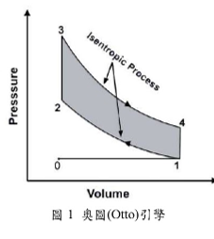
\includegraphics{../Figure/Otto_engine.png}
    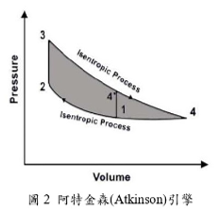
\includegraphics{../Figure/atkinson_engine.png}
\end{center}

\paragraph{解答。}
\textbf{(A)}
\begin{align*}
W_{\text{total}} &= W_{3 \to 4} + W_{1 \to 2} \quad \text{因為 } 1 \to 2 \text{ 與 } 3 \to 4 \text{ 為\zh{絕熱}，} \\
&= - (\Delta U_{3 \to 4} + \Delta U_{1 \to 2}) \\
&= - nkR (T_4 - T_3 + T_2 - T_1).
\end{align*}

\begin{align*}
Q_{\text{abs}} &= Q_{2 \to 3} \quad \text{因為\zh{等體積}，} \\
&= \Delta U_{2 \to 3} = n k R (T_3 - T_2).
\end{align*}

\begin{align*}
\Rightarrow e_O &= - \frac{T_4 - T_3 + T_2 - T_1}{T_3 - T_2} = 1 - \frac{T_4 - T_1}{T_3 - T_2} \\
&= 1 - \left( \frac{V_2}{V_1} \right)^{\gamma - 1}.
\end{align*}

\vspace{1em}
\textbf{(B)}
\begin{align*}
Q_{\text{abs}} &= k R (T_3 - T_2). \\
W_{\text{total}} &= W_{1 \to 2} + W_{3 \to 4} + W_{4 \to 1} \\
&= - kR (T_4 - T_3 + T_2 - T_1) + P_1 (V_1 - V_4).
\end{align*}

\begin{align*}
e_A &= \left[ 1 - \frac{T_4 - T_1}{T_3 - T_2} \right] + \frac{P_1(V_1 - V_4)}{n k R (T_3 - T_2)} \\
&= 1 - \frac{P_1 V_4 - P_1 V_1}{V_L (P_3 - P_2)} + \frac{1}{k} \cdot \frac{P_1 V_4 - P_1 V_1}{V_L (P_3 - P_2)} \\
&= 1 - \left( 1 + \frac{1}{k} \right) \cdot \frac{P_1 V_4 - P_1 V_1}{V_L (P_3 - P_2)} \\
&= 1 - \gamma \cdot \frac{V_4 - V_1}{V_L \left[ \left( \frac{V_4}{V_L} \right)^\gamma - \left( \frac{V_1}{V_L} \right)^\gamma \right]} \\
&= 1 - \gamma \frac{r_E - r_C^{-1}}{r_E^\gamma - r_C^{-\gamma}} = 1 - \gamma r_C^{\gamma - 1} \cdot \frac{r_C r_E - 1}{(r_C r_E)^\gamma - 1}.
\end{align*}

\vspace{1em}
\textbf{(C)}
\begin{align*}
\Rightarrow e_O &= 1 - r_C^{\gamma - 1} \\
e_A &= 1 - r_C^{\gamma - 1} \gamma \frac{x - 1}{x^\gamma - 1}, \quad \text{其中 } x = r_C r_E = \frac{V_4}{V_1} \\
e_A - e_O &= r_C^{\gamma - 1} \left( 1 - \gamma \frac{x - 1}{x^\gamma - 1} \right) = r_C^{\gamma - 1} \frac{(x^\gamma - 1) - \gamma(x - 1)}{x^\gamma - 1}.
\end{align*}

若 $x > 1$，則 $x^\gamma - 1 > 0$。若 $0 < x < 1$ 且 $\gamma > 1$，則 $x^\gamma - 1 < 0$。

令 $f(x) = (x^\gamma - 1) - \gamma(x - 1)$。$f(1) = 0$，$f(0) = \gamma - 1$。
\begin{align*}
f'(x) &= \gamma(x^{\gamma - 1} - 1) < 0 \quad \forall \ 0 < x < 1 \\
f'(x) &> 0 \quad \forall \ x > 1
\end{align*}
\begin{align*}
\Rightarrow \frac{x^\gamma - 1 - \gamma(x - 1)}{x^\gamma - 1} &< 0 \quad \forall \ 0 < x < 1, \\
&> 0 \quad \forall \ x > 1.
\end{align*}
%==============================================================
\section{第二定律}
%==============================================================

\subsection{熱機}

\begin{wrapfigure}{r}[1.5cm]{0.4\textwidth}
  \centering
  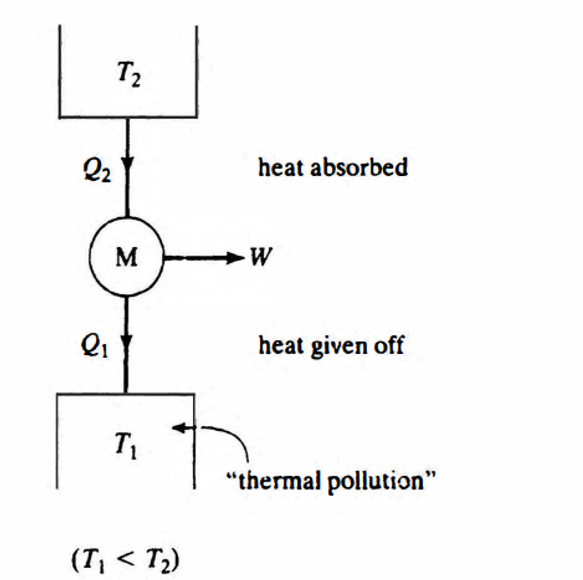
\includegraphics[width=0.4\textwidth]{../Figure/Heat_engine.png}
\end{wrapfigure}

\emph{熱機}是一種循環裝置，它從溫度為 $T_2$ 的高溫熱庫吸收熱 $Q_2$，向溫度為 $T_1<T_2$ 的低溫熱庫釋放熱 $Q_1$，並輸出淨功 $W = Q_2 - Q_1$。其效率為
\[
    e \equiv \frac{W}{Q_2} = 1 - \frac{Q_1}{Q_2}.
\]
普遍的經驗告訴我們，總有某些 $Q_1>0$ 被浪費於低溫熱庫；你永遠無法達到 $e=1$。第二定律即是此一事實的形式化。

%--------------------------------------------------------------
\subsection{公理化敘述}

\paragraph{克勞修斯敘述。} \textit{不可能有任何過程，其唯一效果是將熱從較冷的物體傳遞至較熱的物體。}

\paragraph{克耳文--普朗克敘述。} \textit{沒有任何熱機的效率能達到 $100\%$。}等價地，沒有任何循環裝置能在不產生其他效果的情況下，將熱完全轉換為功。

這兩個敘述是等價的（克勞修斯 $\Leftrightarrow$ 克耳文--普朗克）；每一個都可由另一個藉由串接假想的違反者而證明。此處不再重做該論證。

%--------------------------------------------------------------
\subsection{卡諾熱機與卡諾定理}

\emph{卡諾熱機}是一種如圖所示運作的可逆熱機。它亦可逆向運轉。
\begin{figure}[!htbp]
    \centering
    \begin{subfigure}{0.45\textwidth}
        \centering
        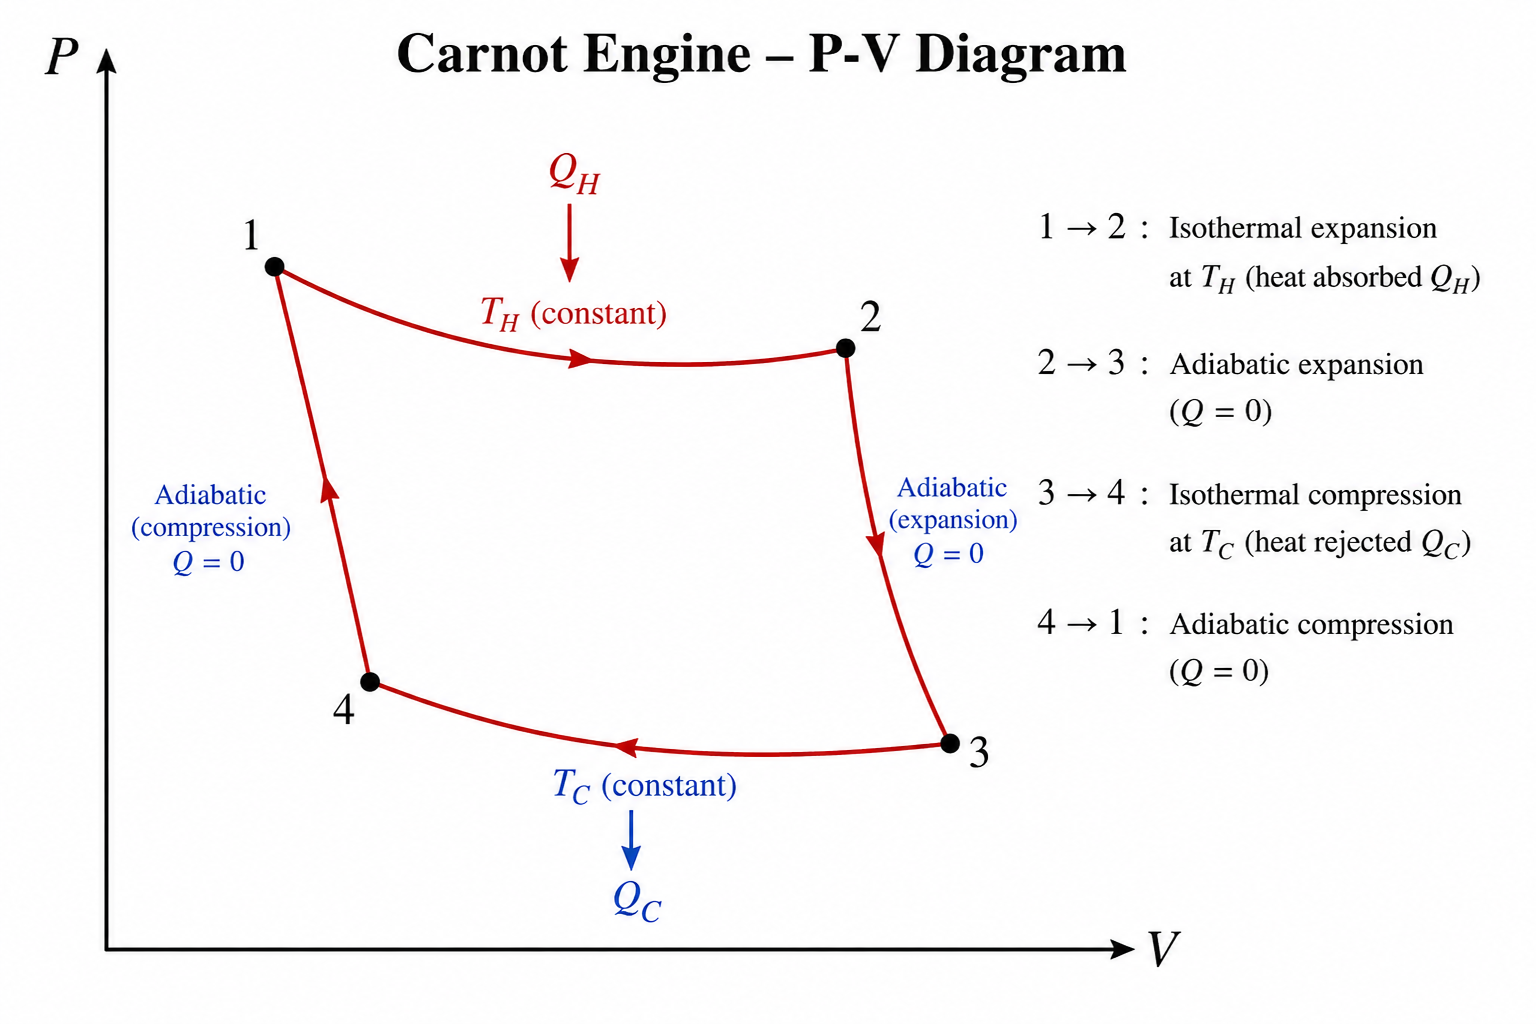
\includegraphics[width=\textwidth]{../Figure/Carnot_engine.png}
        \caption{卡諾熱機。}
    \end{subfigure}
    \hfill
    \begin{subfigure}{0.45\textwidth}
        \centering
        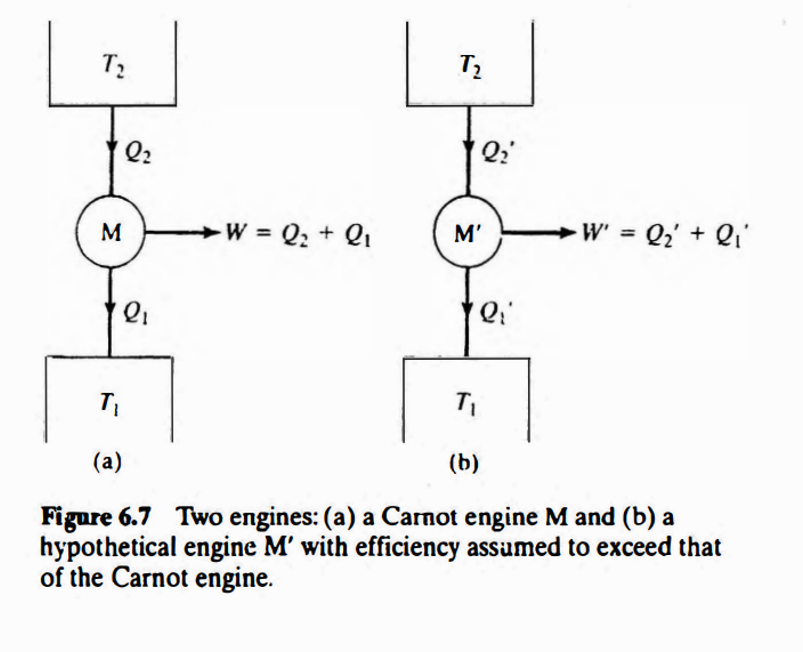
\includegraphics[width=\textwidth]{../Figure/Carnot_theorem.png}
        \caption{卡諾定理證明用之示意圖。}
    \end{subfigure}
\end{figure}

\begin{theorem}
\textbf{（卡諾）}運作於相同兩個熱庫之間的所有卡諾熱機，不論工作物質為何，其效率皆相同。沒有任何熱機能比卡諾熱機更有效率。
\end{theorem}


\paragraph{證明概要。}
假設存在一部效率 $e' > e_{\text{Carnot}}$ 的熱機 $M'$。將 $M'$ 與一部逆向運轉作為冷凍機的卡諾熱機 $M$ 耦合，
並使其大小恰使 $M'$ 的功輸出剛好驅動 $M$。
此組合裝置的淨效果，是在沒有淨功的情況下把一正量的熱從低溫熱庫泵送至高溫熱庫
——這違反了克勞修斯敘述。因此這樣的 $M'$ 並不存在。

注意此定理同時也證明了：不論工作物質為何，\emph{所有}卡諾熱機的效率皆相同。
這可由類似的論證證明：用效率較高的熱機產生功，並用另一部作為冷凍機。

卡諾效率結果只取決於兩個溫度，這可利用理想氣體推導：
\[
    e_{\text{Carnot}} = 1 - \frac{T_1}{T_2}.
\]
事實上，這個關係式可\emph{用來}定義絕對溫標：（選取 $T$ 使得卡諾熱機滿足 $\frac{Q_1}{Q_2} = \frac{T_1}{T_2}$）。

%--------------------------------------------------------------
\subsection{克勞修斯不等式}
我們將提出一個引理，它對於以「卡諾循環切片」進行此不等式的「古典」證明至為關鍵；
該證明此處不予呈現，而置於附錄中。
\begin{lemma}
對任何熱力學物質而言，內能與壓力透過現代熱力學狀態方程式與絕對溫度 $T$ 相關聯：
\[
\left(\frac{\partial U}{\partial V}\right)_T + P = T\left(\frac{\partial P}{\partial T}\right)_V
\]
\end{lemma}

我們同樣將此引理的證明留至附錄。現在，敘述克勞修斯不等式：

\begin{theorem}
    對任何循環過程，
    \begin{enumerate}
        \item 對可逆循環，$\displaystyle \oint \frac{\dbar Q_{\text{rev}}}{T} = 0$。
        \item 對不可逆循環，$\displaystyle \oint \frac{\dbar Q_{\text{irr}}}{T} < 0$。
    \end{enumerate}
\end{theorem}


\begin{proof}
令一系統經歷一個任意的、可能為不可逆的循環過程。
在此循環中，系統在不同的邊界溫度 $T_{\text{ext}}$ 下與其環境交換不等量的熱 $\delta Q$。

\textbf{1. 設置。}

我們引入一個維持在固定絕對溫度 $T_0$ 的巨大主熱庫。
我們亦設想：對任意 $T_{\text{ext}}$ 值，都存在一部運作於主熱庫與 $T_{\text{ext}}$ 之間的
\textbf{可逆輔助卡諾熱機}。

每當系統在 $T_{\text{ext}}$ 吸收 $\delta Q$ 時，一部輔助卡諾熱機便從 $T_0$ 的主熱庫汲取 $\delta Q_0$，
並向 $T_{\text{ext}}$ 送回 $\delta Q$ 以抵消該吸收。

由於這些輔助熱機完全可逆地運作，它們嚴格滿足絕對熱力學溫度比：
\[
\frac{\delta Q_0}{T_0} = \frac{\delta Q}{T_{\text{ext}}} \implies \delta Q_0 = T_0 \frac{\delta Q}{T_{\text{ext}}}
\]

\textbf{2. 對整個循環積分。}

我們讓主系統完成一個完整的封閉巨觀循環，精確地回到其初始狀態，
並對整個合併的宇宙（由主系統與所有輔助熱機組成）套用熱力學第一定律。

由能量守恆，此合併系統所執行的總淨機械功 $W_{\text{net}}$
必須恰好等於從單一主熱庫所抽取的總淨熱 $Q_0$：
\[
W_{\text{net}} = Q_0 = \oint \delta Q_0
\]
將我們對 $\delta Q_0$ 的關係式代入循環積分得：
\[
W_{\text{net}} = \oint T_0 \frac{\delta Q}{T_{\text{ext}}}= T_0 \oint \frac{\delta Q}{T_{\text{ext}}}
\]
由於主熱庫溫度 $T_0$ 在整個過程中保持嚴格固定，它可被提出積分之外。

\textbf{3. 套用第二定律。}
根據\textbf{熱力學第二定律的克耳文--普朗克敘述}，
要建造一部循環運作、且僅與單一熱庫交換熱卻產生淨正功的裝置，在物理上是不可能的。
若過程為不可逆，則淨功必嚴格小於零。若過程完全可逆，則淨功恰為零。因此：
\[
W_{\text{net}} \le 0
\]
將此約束與我們的能量平衡式結合得：
\[
T_0 \oint \frac{\delta Q}{T_{\text{ext}}} \le 0, \qquad \oint \frac{\delta Q}{T_{\text{ext}}} \le 0
\]
\end{proof}

\begin{center}
  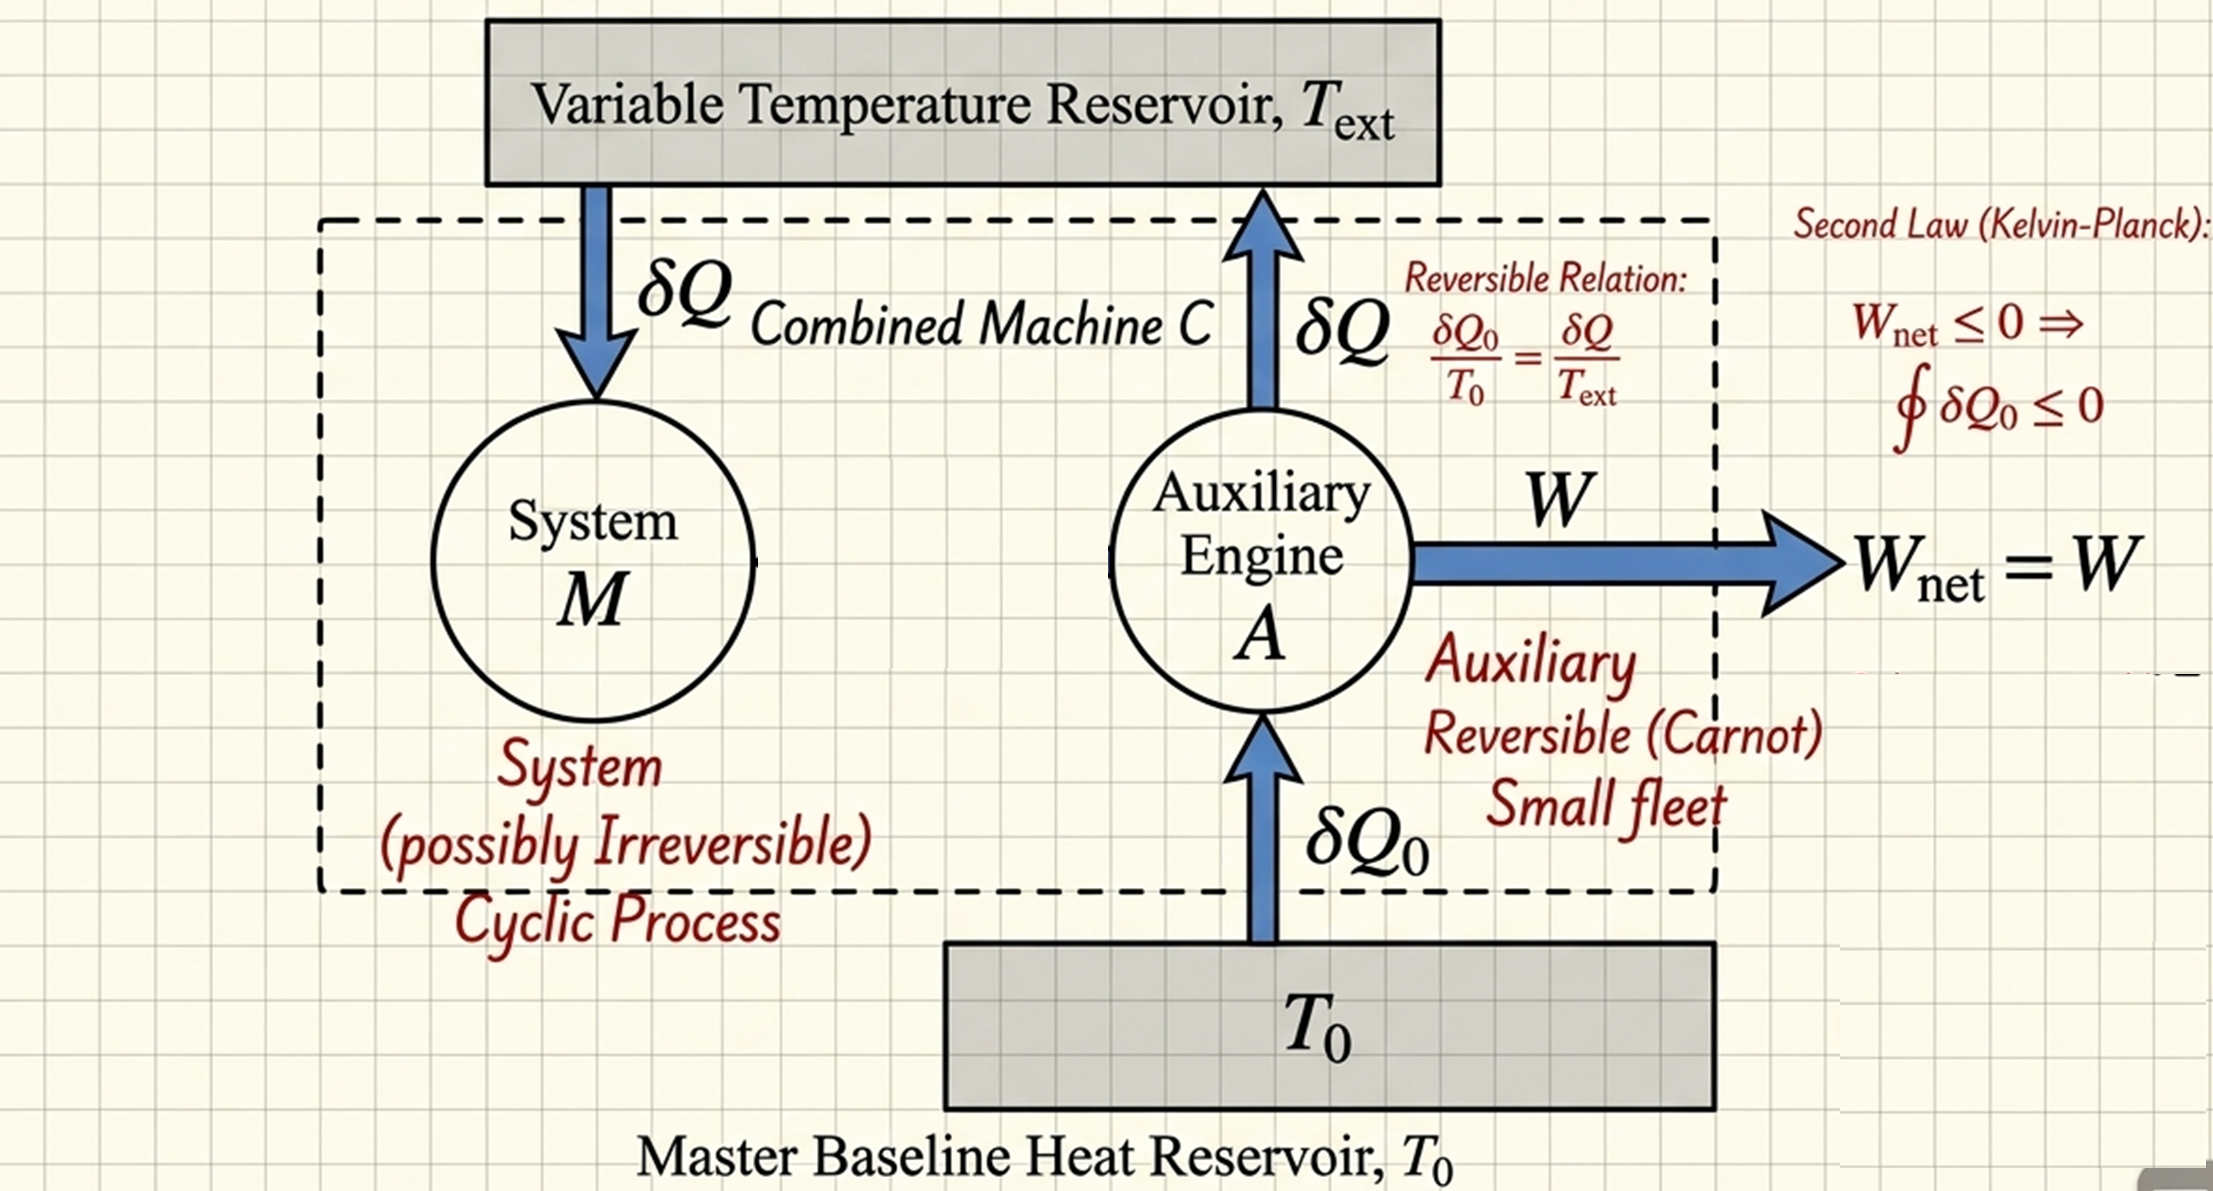
\includegraphics[width=0.8\textwidth]{../Figure/clausius_proof.png}
\end{center}


此證明實際上同時證明了可逆與不可逆兩種情形。看來古典的「卡諾循環切片」證明
其實並非必要。儘管如此，為求完整我們仍將其呈現於附錄中。見第 \ref{sec:clausius_inequality} 節。
%--------------------------------------------------------------
\subsection{熵}

由於沿任何封閉循環 $\oint \dbar Q_{\text{rev}}/T = 0$，微分形式 $\dbar Q_{\text{rev}}/T$ 是\emph{恰當的}。
因此必存在一個狀態函數 $S$——即\emph{熵}——其微分為
\[
    \boxed{\,\dd S = \frac{\dbar Q_{\text{rev}}}{T}\,}.
\]
差值 $S_B - S_A$ 可藉由沿\emph{任何}從 $A$ 到 $B$ 的可逆路徑對 $\dbar Q/T$ 積分而求得；其結果與路徑無關。
不過，在此階段 $S$ 的絕對值仍未定義。（這需要第三定律，即對完美晶體當 $T \to 0$ 時 $S \to 0$，此處我們並不需要。）

%==============================================================
\section{$T\dd S$ 方程式}
%==============================================================
我們其實在前面已經提出過這個引理，並在附錄中以不使用恰當性的方式予以證明，
但此處我們將提供一個利用 $\dd S$ 恰當性的較優雅版本，並附上一個對應於 $H$ 的版本。
\subsection{由恰當性得到的一個有用引理}

熵是狀態函數，故 $\dd S$ 是恰當的。從
\[
    \dd S = \frac{\dbar Q}{T} = \frac{\dd U}{T} + \frac{P}{T}\,\dd V
          = \frac{C_V}{T}\,\dd T + \frac{1}{T}\!\left[P + \pa{U}{V}_T\right]\!\dd V
\]
出發，恰當性要求 $\dd T$ 與 $\dd V$ 兩係數的混合偏導數相等：
\[
    \pd{}{V}\!\left(\frac{C_V}{T}\right)_T = \pd{}{T}\!\left(\frac{1}{T}\!\left[P + \pa{U}{V}_T\right]\right)_V.
\]
展開並化簡，
\[
    0 = \frac{1}{T}\!\left[\pa{P}{T}_V + \pd{^{2}U}{T\,\partial V}\right] - \frac{1}{T^{2}}\!\left(P + \pa{U}{V}_T\right),
\]
整理後得到非常有用的關係式
\[
    \boxed{\,\pa{U}{V}_T = T\,\pa{P}{T}_V - P\,}.
\]
從 $\dd S = (\dd H - V\,\dd P)/T$ 出發的完全類似的計算給出
\[
    \boxed{\,\pa{H}{P}_T = -T\,\pa{V}{T}_P + V\,}.
\]

\paragraph{這些為何有用。}
$\pa{U}{V}_T$ 與 $\pa{H}{P}_T$ 這兩個偏導數出了名地難以計算——焦耳與焦耳--湯姆森告訴我們它們對理想氣體會消失，但對固體與液體我們完全無從下手。有了這些引理，我們所需的只是\emph{可量測的}力學響應：熱膨脹係數 $\beta = \pa{V}{T}_P/V$ 與壓力--溫度導數 $\pa{P}{T}_V$。這兩者都是例行的桌上型量測。

\paragraph{習題。}
\zh{
(A) 卡諾熱機在兩個不同溫度的熱庫（heat reservoir）循環運作時，其過程均為可逆。

考慮如圖 1 所示的卡諾熱機，熱機由二可逆等溫過程（$a \to b$；$c \to d$）和二可逆絕熱過程（$b \to c$；$d \to a$）組成。
試計算每一過程中熱機內氣體（假設為 $n$ 莫耳的理想氣體）熵的變化量。

（以氣體壓力 $P$、體積 $V$、溫度 $T$ 和其他相關常數表示。）（8 分）

(B) 現考慮兩個具有相同熱容量 $C$ 的物質，其起始溫度分別為 $T_1$ 和 $T_2$。今有一卡諾熱機

以此二物質為其低溫和高溫熱庫，並假設卡諾熱機運行一循環時，二熱庫的溫度變化，

遠小於其個別的溫度值。

問此二物質的最終溫度為何？過程中卡諾熱機可作的最大功為何？（9 分）

(C) 現考慮三個具有相同熱容量 $C$ 的物質，其起始溫度分別為
$T_1 = 100\,\mathrm{K}$、
$T_2 = 300\,\mathrm{K}$
和
$T_3 = 300\,\mathrm{K}$。

假設我們可以利用前述的卡諾熱機在物質 1 和 2 之間運轉並輸出功，並以另一在物質 1 和物質 3 之間運轉的卡諾熱機，將所輸出的功完全用於提高物質 3 的溫度。問：

(i) 物質 1 所能達到的最低溫度 $T_L$ 為何？（2 分）

(ii) 物質 3 可以達到的最高溫度 $T_H$ 為何？（6 分）
}
\paragraph{解答。}
\textbf{(A)} \\
在卡諾循環中，所有 4 個過程皆為可逆。因此，氣體在每一步的熵變化 $\Delta S$ 由下式給出：
\[ \Delta S = \int_{i}^{f} \frac{dQ}{T} \]
對絕熱過程（$b \to c$ 與 $d \to a$）：
\[ \Delta S_{b \to c} = 0, \quad \Delta S_{d \to a} = 0 \quad (\text{因為 } dQ = 0) \]
對等溫過程（$a \to b$ 與 $c \to d$）：
\[ dQ = dU + P\,dV = P\,dV = \frac{nRT}{V}\,dV \]
\[ \Rightarrow \Delta S = \int_{V_i}^{V_f} \frac{nRT}{TV}\,dV = nR \ln \frac{V_f}{V_i} \]
因此，
\[ \Delta S_{a \to b} = nR \ln \frac{V_b}{V_a}, \quad \Delta S_{c \to d} = nR \ln \frac{V_d}{V_c} \]
注意，由絕熱過程的性質（$TV^{\gamma-1} = \text{const}$），我們有：
\begin{align*}
T_H V_a^{\gamma-1} &= T_L V_d^{\gamma-1} \\
T_H V_b^{\gamma-1} &= T_L V_c^{\gamma-1}
\end{align*}
兩式相除得：
\[ \left(\frac{V_a}{V_b}\right)^{\gamma-1} = \left(\frac{V_d}{V_c}\right)^{\gamma-1} \implies \frac{V_a}{V_b} = \frac{V_d}{V_c} \implies \frac{V_b}{V_a} = \frac{V_c}{V_d} \]
因此，第二個等溫過程中的熵變化為：
\[ \Delta S_{c \to d} = nR \ln \frac{V_d}{V_c} = -nR \ln \frac{V_c}{V_d} = -nR \ln \frac{V_b}{V_a} = -\Delta S_{a \to b} \]
（這與 $S$ 為狀態變數的事實相符，故 $\Delta S_{\text{cycle}} = 0$。）

\vspace{1em}
\textbf{(B)} \\
令兩熱庫的起始溫度為 $T_{1,i}$ 與 $T_{2,i}$，其中 $T_{2,i} > T_{1,i}$。令 $\rho = \frac{V_b}{V_a}$ 為膨脹比。
對一個無窮小循環，與熱庫交換的熱為：
\[ dQ_{\text{hot}} = -dQ_{a \to b} \implies C\,dT_2 = -nR T_2 \ln \rho \]
\[ dQ_{\text{cold}} = dQ_{c \to d, \text{rejected}} \implies C\,dT_1 = nR T_1 \ln \rho \]
整理這些式子得：
\[ -\frac{dT_2}{T_2} = \frac{nR}{C}\ln \rho = \frac{dT_1}{T_1} \]
對許多循環積分，直至最終平衡態 $T_{1,f} = T_{2,f} = T_f$：
\[ \int_{T_{1,i}}^{T_f} \frac{dT_1}{T_1} = -\int_{T_{2,i}}^{T_f} \frac{dT_2}{T_2} \]
\[ \Rightarrow \ln \frac{T_f}{T_{1,i}} = -\ln \frac{T_f}{T_{2,i}} = \ln \frac{T_{2,i}}{T_f} \]
\[ \Rightarrow T_f^2 = T_{1,i} T_{2,i} \implies T_f = \sqrt{T_{1,i} T_{2,i}} \]
（以題目給定的參數表示，最終溫度為 $\sqrt{T_1 T_2}$。）

熱機所做的最大功 $W$ 可利用能量守恆（$W = -\Delta U_{\text{reservoirs}}$）求得：
\begin{align*}
W &= -C(T_f - T_{2,i}) - C(T_f - T_{1,i}) \\
  &= C(T_{1,i} + T_{2,i} - 2T_f) \\
  &= C\left(T_{1,i} + T_{2,i} - 2\sqrt{T_{1,i}T_{2,i}}\right) = C\left(\sqrt{T_{2,i}} - \sqrt{T_{1,i}}\right)^2
\end{align*}

\vspace{1em}
\textbf{(C)} \\
令熱機 1 運作於 $T_2$ 與 $T_1$ 之間，從 $T_2$ 抽取熱 $Q_h$，向 $T_1$ 排放熱，並產生功 $W = \eta_1 Q_h$。
令熱機 2（作為熱泵）運作於 $T_1$ 與 $T_3$ 之間，利用全部的功 $W$ 把熱從 $T_1$ 泵送至 $T_3$。其性能係數為 $1/\eta_2$。
傳遞至 $T_3$ 的熱為 $Q_3 = W/\eta_2 = (\eta_1/\eta_2)Q_h$。
熱泵從 $T_1$ 抽取的熱為 $Q_{\text{extracted}} = Q_3 - W = \eta_1\left(\frac{1}{\eta_2}-1\right)Q_h$。

\textbf{(i)} 加入物質 1 的淨熱為：
\[ dQ_1 = (1-\eta_1)Q_h - \eta_1\left(\frac{1}{\eta_2}-1\right)Q_h = \left(1 - \frac{\eta_1}{\eta_2}\right)Q_h \]
由於 $T_2 \downarrow$ 且 $T_3 \uparrow$，我們有 $\eta_1 \downarrow$ 且 $\eta_2 \uparrow$。起初 $T_2 = T_3 = 300\,\text{K}$，故 $\eta_1 = \eta_2$。
隨著過程進行，$\eta_1 \le \eta_2$，這意味著 $1 - \frac{\eta_1}{\eta_2} \ge 0$。
因此 $dQ_1 \ge 0$。由於熱持續加入物質 1，其溫度永不下降。
所以，最低溫度即為其初始溫度：
\[ T_{1,\text{min}} = 100\,\text{K} \]

\textbf{(ii)} 對於三個物質所構成的系統，假設所有過程皆為可逆，總熵變化為零：
\[ dS_1 + dS_2 + dS_3 = \frac{dQ_1}{T_1} + \frac{dQ_2}{T_2} + \frac{dQ_3}{T_3} = 0 \]
\[ \Rightarrow C\left(\frac{dT_1}{T_1} + \frac{dT_2}{T_2} + \frac{dT_3}{T_3}\right) = 0 \implies d(\ln(T_1 T_2 T_3)) = 0 \]
\[ \Rightarrow T_1 T_2 T_3 = \text{const} = 100 \times 300 \times 300 = 9 \times 10^6 \]
由能量守恆，與環境之間沒有淨熱或淨功的交換：
\[ dQ_1 + dQ_2 + dQ_3 = 0 \implies C(dT_1 + dT_2 + dT_3) = 0 \]
\[ \Rightarrow T_1 + T_2 + T_3 = \text{const} = 100 + 300 + 300 = 700 \]
為使 $T_3$ 最大化，$T_2$ 必須下降，直到熱機 1 不再能抽取功為止，此時 $T_1 = T_2 = T$。
將 $T_1 = T_2 = T$ 代入守恆方程式：
\[ 2T + T_3 = 700 \implies T_3 = 700 - 2T \]
\[ T^2 T_3 = 9 \times 10^6 \implies T^2(700 - 2T) = 9 \times 10^6 \]
\[ 2T^3 - 700T^2 + 9 \times 10^6 = 0 \implies T^3 - 350T^2 + 4.5 \times 10^6 = 0 \]
觀察可知 $T = 150\,\text{K}$ 為一根（$150^3 - 350(150^2) + 4.5 \times 10^6 = 3375000 - 7875000 + 4500000 = 0$）。
因此 $T_3 = 700 - 2(150) = 400\,\text{K}$。
物質 3 所能達到的最高溫度為：
\[ T_H = 400\,\text{K} \]

%--------------------------------------------------------------
\subsection{三個 $T\dd S$ 方程式}

我們可將 $\dd S$ 表為 $P,V,T$ 中任兩者的函數。共有三對組合，故有三種形式：
\begin{align}
    T\,\dd S &= n C_V\,\dd T + T\,\pa{P}{T}_V\,\dd V, \label{eq:TdS1}\\[4pt]
    T\,\dd S &= n C_P\,\dd T - T\,\pa{V}{T}_P\,\dd P, \label{eq:TdS2}\\[4pt]
    T\,\dd S &= n C_P\,\pa{T}{V}_P\,\dd V + n C_V\,\pa{T}{P}_V\,\dd P. \label{eq:TdS3}
\end{align}
推導很直接：在第一定律中寫下 $\dbar Q = T\,\dd S$，然後將 $(P,V,T)$ 中你想用的那一對作為自由變數（第三者透過狀態方程式與上述引理消去）。

\paragraph{應用：理想氣體的熵變化。}
將 $\pa{P}{T}_V = nR/V$ 代入~\eqref{eq:TdS1}，
\[
    T\,\dd S = n C_V\,\dd T + \frac{nRT}{V}\,\dd V.
\]
兩邊同除以 $T$ 再積分（這一步稍嫌不嚴謹：我們假設 $C_V$ 為常數，這對 IPhO 範圍內的單原子與雙原子理想氣體是沒問題的），
\[
    \boxed{\,\Delta S = n C_V \ln\!\frac{T}{T_0} + nR \ln\!\frac{V}{V_0}\,}.
\]
此公式是奧林匹亞熵問題的主力工具。注意它僅適用於理想氣體。


%==============================================================
\section{熱力學勢}
%==============================================================

\subsection{四種能量}

我們已遇過兩個具有能量單位的狀態函數，$U$ 與 $H$。現在再引入兩個：
\begin{align*}
    A &\equiv U - TS \qquad \text{（亥姆霍茲自由能）},\\
    G &\equiv H - TS \qquad \text{（吉布斯自由能）}.
\end{align*}
這四者皆為狀態函數，其微分（代入 $\dbar Q_{\text{rev}}=T\,\dd S$ 與 $\dbar W_{\text{rev}}=-P\,\dd V$ 後）為
\[
    \boxed{\begin{aligned}
        \dd U &= T\,\dd S - P\,\dd V, \vphantom{\left(\frac{\partial U}{\partial S}\right)_V} \\
        \dd H &= T\,\dd S + V\,\dd P, \vphantom{\left(\frac{\partial H}{\partial S}\right)_P} \\
        \dd A &= -S\,\dd T - P\,\dd V, \vphantom{\left(\frac{\partial A}{\partial T}\right)_V} \\
        \dd G &= -S\,\dd T + V\,\dd P, \vphantom{\left(\frac{\partial G}{\partial T}\right)_P}
    \end{aligned}}
    \quad\implies\quad
    \begin{aligned}
        \left(\frac{\partial U}{\partial S}\right)_V &= T, & \left(\frac{\partial U}{\partial V}\right)_S &= -P, \\[1ex]
        \left(\frac{\partial H}{\partial S}\right)_P &= T, & \left(\frac{\partial H}{\partial P}\right)_S &= V, \\[1ex]
        \left(\frac{\partial A}{\partial T}\right)_V &= -S, & \left(\frac{\partial A}{\partial V}\right)_T &= -P, \\[1ex]
        \left(\frac{\partial G}{\partial T}\right)_P &= -S, & \left(\frac{\partial G}{\partial P}\right)_T &= V.
    \end{aligned}
\]
注意我們之所以能像這樣「讀出」係數，是因為現在這些微分都是恰當的，不像原本的 $\dd U = \dbar Q + \dbar W$。
依各式右側的變數讀出每個公式：$U(S,V)$、$H(S,P)$、$A(T,V)$、$G(T,P)$。
雖然現在我們有四個變數 $\{P,V,T,S\}$，自由度仍為 2。

\paragraph{為何引入 $A$ 與 $G$？}
\begin{itemize}
    \item 當 $T$ 與 $V$ 固定時，$A$ 在平衡態取極小值。
    \item 當 $T$ 與 $P$ 固定時，$G$ 在平衡態取極小值。
\end{itemize}

%--------------------------------------------------------------
\subsection{馬克士威關係式}

四個勢中的每一個都是狀態函數，故其微分皆為恰當，任兩個係數的混合偏導數相等。例如，由 $\dd U = T\,\dd S - P\,\dd V$，
\[
    \pa{T}{V}_S = -\pa{P}{S}_V.
\]
對全部四個勢都這麼做，得到四條\emph{馬克士威關係式}：
\[
    \boxed{\begin{aligned}
        \pa{T}{V}_S &= -\pa{P}{S}_V \qquad (\text{由 } \dd U),\\[4pt]
        \pa{T}{P}_S &= \phantom{-}\pa{V}{S}_P \qquad (\text{由 } \dd H),\\[4pt]
        \pa{S}{V}_T &= \phantom{-}\pa{P}{T}_V \qquad (\text{由 } \dd A),\\[4pt]
        \pa{S}{P}_T &= -\pa{V}{T}_P \qquad (\text{由 } \dd G).
    \end{aligned}}
\]
後兩條在解題時遠為有用——你會在幾乎每一次 $T\dd S$ 的計算中看到它們出現。

%==============================================================
\section{多相與多成分系統}
%==============================================================

\subsection{加入組成變數}

到目前為止，每個系統都是單一化學成分的單一相。一旦允許更多，變數數目便增加：對於兩相（譬如同一物質的液相與氣相），總莫耳數 $n_1 + n_2$ 是固定的，但兩相之間的分配則是一個新的自由度。

以 $G$ 為例，對一個兩相系統，
\[
    \dd G = -S\,\dd T + V\,\dd P + \pa{G}{n_1}_{T,P,n_2}\dd n_1 + \pa{G}{n_2}_{T,P,n_1}\dd n_2.
\]
由於總量 $n_1 + n_2$ 守恆，$\dd n_2 = -\dd n_1$，末兩項合併為
\[
    \dd G = -S\,\dd T + V\,\dd P + (\mu_1 - \mu_2)\,\dd n_1,
\]
其中
\[
    \mu_i \equiv \pa{G}{n_i}_{T,P,n_{j\neq i}}
\]
是成分（或相）$i$ 的\emph{化學勢}。化學勢是在固定 $T,P$ 與其他成分下，每加入一莫耳 $i$ 所引起的 $G$ 變化。

%--------------------------------------------------------------
\subsection{吉布斯能與自發性}

我們現在來證成標準化學教科書的論述：
\begin{quote}
\textit{在固定 $T$ 與 $P$ 下，自發過程滿足 $\Delta G < 0$。}
\end{quote}

\paragraph{設置。} 考慮一個與固定 $T$ 和 $P$ 之環境保持熱接觸與力學接觸的封閉系統。假設某過程從環境吸收熱 $\Delta Q$。環境因其體量龐大而可逆地變化，故其熵變化為
\[
    \Delta S_{\text{sur}} = -\frac{\Delta Q}{T}.
\]
\paragraph{系統的第一定律。} 假設功純粹為 $PV$ 功，且系統的路徑可化為可逆，
\[
    \Delta Q = \Delta U + P\,\Delta V.
\]
\paragraph{對設想之回程套用克勞修斯。} 現在設想進行一個（假想的）可逆過程，使系統回到其初始狀態。對該不可逆循環（不可逆正向 + 可逆逆向）套用克勞修斯不等式，
\[
    \Delta Q < T\,\Delta S_{\text{sys}}.
\]
（當且僅當正向步驟原本就可逆時取等號。）

\paragraph{綜合起來。} 將兩者結合：
\[
    \Delta U + P\,\Delta V < T\,\Delta S
    \;\;\Longleftrightarrow\;\;
    \Delta U + P\,\Delta V - T\,\Delta S < 0
    \;\;\Longleftrightarrow\;\;
    \Delta(U + PV - TS) < 0,
\]
其中最後一步用到 $T$ 與 $P$ 保持固定。組合 $U + PV - TS$ 恰為 $G$，故對任何在固定 $T$ 與 $P$ 下的自發過程，
\[
    \boxed{\,\Delta G < 0\,}
\]
成立，並於平衡時 $\Delta G = 0$。

%==============================================================
\section{相平衡與克拉佩龍方程式}
%==============================================================

\subsection{克拉佩龍方程式}

考慮同一物質的兩相（譬如 $1 =$ 液相，$2 =$ 氣相）在某溫度 $T$ 與壓力 $P$ 下共存。令 $n_1,n_2$ 為兩相的莫耳數，其中 $n_1+n_2$ 固定。若有少量 $-\dd n_1 = \dd n_2 > 0$ 使相~$1$ 轉變為相~$2$，則吉布斯能變化為
\[
    \dd G = (\mu_2 - \mu_1)\,\dd n_1.
\]
在平衡時對任意 $\dd n_1$ 皆有 $\dd G = 0$，這迫使
\[
    \boxed{\,\mu_1(T,P) = \mu_2(T,P)\,}.
\]
這就是\emph{相平衡條件}：沿 $(T,P)$ 平面上的共存曲線，兩相的化學勢相等。

\paragraph{沿共存曲線滑動。}
現在假設我們把 $T\to T+\dd T$ 與 $P\to P+\dd P$ 變化，使得兩相持續共存。那麼 $\mu_1=\mu_2$ 必須維持，即 $\dd\mu_1=\dd\mu_2$。利用 $\dd G = -S\,\dd T + V\,\dd P$ 的莫耳形式，
\[
    \dd\mu_1 = -s_1\,\dd T + v_1\,\dd P
    = -s_2\,\dd T + v_2\,\dd P
    = \dd\mu_2,
\]
其中小寫的 $s_i, v_i$ 是相 $i$ 的莫耳熵與莫耳體積。解出 $\dd P/\dd T$，
\[
    \boxed{\,\frac{\dd P}{\dd T} = \frac{s_2 - s_1}{v_2 - v_1} = \frac{\Delta H_{\text{trans}}}{T\,\Delta v}\,}.
\]
最後一個等號用到 $T\,\Delta s = \Delta H_{\text{trans}}$，即該轉變的莫耳潛熱（因轉變在固定 $T$ 與 $P$ 下發生而成立）。這就是\textbf{克拉佩龍方程式}。

%--------------------------------------------------------------
\subsection{克勞修斯--克拉佩龍方程式}

對液--氣轉變，我們再做兩個進一步的近似：
\begin{enumerate}[label=(\roman*)]
    \item 氣相表現如理想氣體，故 $v_{\text{vap}} = RT/P$；
    \item 氣相體積遠大於液相體積，故 $\Delta v \approx v_{\text{vap}}$。
\end{enumerate}
代入克拉佩龍方程式，
\[
    \frac{\dd P}{\dd T} = \frac{\Delta H}{T\,(RT/P)} = \frac{\Delta H}{R}\,\frac{P}{T^{2}}.
\]
分離變數並積分（假設 $\Delta H$ 在該溫度範圍內近似為常數），
\[
    \int_{P_0}^{P} \frac{\dd P'}{P'} = \frac{\Delta H}{R}\int_{T_0}^{T} \frac{\dd T'}{T'^{2}}
    \;\;\Longrightarrow\;\;
    \boxed{\,\ln\!\frac{P}{P_0} = -\frac{\Delta H}{R}\!\left(\frac{1}{T} - \frac{1}{T_0}\right)\,},
\]
或以指數形式表示，
\[
    P = P_0 \exp\!\left[-\frac{\Delta H}{R}\!\left(\frac{1}{T} - \frac{1}{T_0}\right)\right].
\]
這就是\textbf{克勞修斯--克拉佩龍方程式}。
% =============================================================
%  classical_thermodynamics.tex 結束
% =============================================================
